\documentclass{beamer}\usepackage{graphicx, color}
%% maxwidth is the original width if it is less than linewidth
%% otherwise use linewidth (to make sure the graphics do not exceed the margin)
\makeatletter
\def\maxwidth{ %
  \ifdim\Gin@nat@width>\linewidth
    \linewidth
  \else
    \Gin@nat@width
  \fi
}
\makeatother

\definecolor{fgcolor}{rgb}{0.2, 0.2, 0.2}
\newcommand{\hlnumber}[1]{\textcolor[rgb]{0,0,0}{#1}}%
\newcommand{\hlfunctioncall}[1]{\textcolor[rgb]{0.501960784313725,0,0.329411764705882}{\textbf{#1}}}%
\newcommand{\hlstring}[1]{\textcolor[rgb]{0.6,0.6,1}{#1}}%
\newcommand{\hlkeyword}[1]{\textcolor[rgb]{0,0,0}{\textbf{#1}}}%
\newcommand{\hlargument}[1]{\textcolor[rgb]{0.690196078431373,0.250980392156863,0.0196078431372549}{#1}}%
\newcommand{\hlcomment}[1]{\textcolor[rgb]{0.180392156862745,0.6,0.341176470588235}{#1}}%
\newcommand{\hlroxygencomment}[1]{\textcolor[rgb]{0.43921568627451,0.47843137254902,0.701960784313725}{#1}}%
\newcommand{\hlformalargs}[1]{\textcolor[rgb]{0.690196078431373,0.250980392156863,0.0196078431372549}{#1}}%
\newcommand{\hleqformalargs}[1]{\textcolor[rgb]{0.690196078431373,0.250980392156863,0.0196078431372549}{#1}}%
\newcommand{\hlassignement}[1]{\textcolor[rgb]{0,0,0}{\textbf{#1}}}%
\newcommand{\hlpackage}[1]{\textcolor[rgb]{0.588235294117647,0.709803921568627,0.145098039215686}{#1}}%
\newcommand{\hlslot}[1]{\textit{#1}}%
\newcommand{\hlsymbol}[1]{\textcolor[rgb]{0,0,0}{#1}}%
\newcommand{\hlprompt}[1]{\textcolor[rgb]{0.2,0.2,0.2}{#1}}%

\usepackage{framed}
\makeatletter
\newenvironment{kframe}{%
 \def\at@end@of@kframe{}%
 \ifinner\ifhmode%
  \def\at@end@of@kframe{\end{minipage}}%
  \begin{minipage}{\columnwidth}%
 \fi\fi%
 \def\FrameCommand##1{\hskip\@totalleftmargin \hskip-\fboxsep
 \colorbox{shadecolor}{##1}\hskip-\fboxsep
     % There is no \\@totalrightmargin, so:
     \hskip-\linewidth \hskip-\@totalleftmargin \hskip\columnwidth}%
 \MakeFramed {\advance\hsize-\width
   \@totalleftmargin\z@ \linewidth\hsize
   \@setminipage}}%
 {\par\unskip\endMakeFramed%
 \at@end@of@kframe}
\makeatother

\definecolor{shadecolor}{rgb}{.97, .97, .97}
\definecolor{messagecolor}{rgb}{0, 0, 0}
\definecolor{warningcolor}{rgb}{1, 0, 1}
\definecolor{errorcolor}{rgb}{1, 0, 0}
\newenvironment{knitrout}{}{} % an empty environment to be redefined in TeX

\usepackage{alltt}
\usepackage{beamerthemeDresden} 
\usepackage[english]{babel}
\usepackage{amsmath,amssymb}
\usepackage[latin1]{inputenc}
\usepackage{palatino}
\usepackage{graphicx}
\usepackage{subfigure}
\usepackage{pgf}
\usepackage{relsize}
\def\bs{\mathbf{s}}
\def\bit{\begin{itemize}}
\def\eit{\end{itemize}}
\IfFileExists{upquote.sty}{\usepackage{upquote}}{}
\begin{document}


\title[]{Spatial Plot-based Methods for Estimating Abundance}

\author[Jay M. Ver Hoef]{Jay Ver Hoef} 

\institute[NOAA National Marine Mammal Lab]
{
	\normalsize NOAA National Marine Mammal Lab \\
	NOAA Fisheries \\
	International Arctic Research Center \\
	Fairbanks, Alaska, USA\\
	\vspace{0.1cm}
}
\date[05/17/13]{}
 
\maketitle
 
% very important to use option [fragile] for frames containing code output!
%-------------------------------------------------------------------------------
%                        OUTLINE
%-------------------------------------------------------------------------------
 
\section{Introduction}
\subsection{Outline}
\begin{frame}[fragile]
	\begin{tabular} {p{5.8cm} p{3.8cm}}
	{
		\begin{center}
		\bit
			\item Introduction
				\vspace{0.2cm}       
			\item Review of Spatial Statistics         
				\vspace{0.2cm} 
			\item Block Kriging    
				\vspace{0.2cm}      
			\item Block Prediction for Finite Populations on a Grid   
				\vspace{0.2cm}      
			\item Block Prediction for Finite Populations of Irregularly-Spaced Plots 
		\eit
	\end{center}
	} &
	{
		\vspace{.1cm}
%		\hspace{-.7cm}
		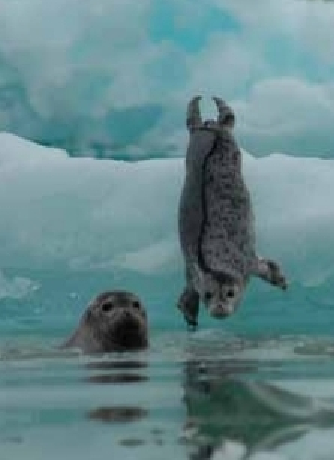
\includegraphics[width=4.0cm]{figure/SealInWater.pdf} 
	}
	\end{tabular}
\end{frame}

%-------------------------------------------------------------------------------
%                        Aerial Photos for Seals
%-------------------------------------------------------------------------------

\begin{frame}[fragile]
\frametitle{Aerial Photos for Seals}
	\begin{tabular} {p{5.0cm} p{5.0cm}}
	

			\vspace{0cm}
			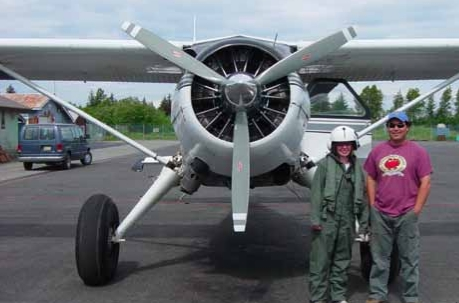
\includegraphics[width=4.6cm]{figure/airplane.jpeg}  &
			\vspace{1cm}
			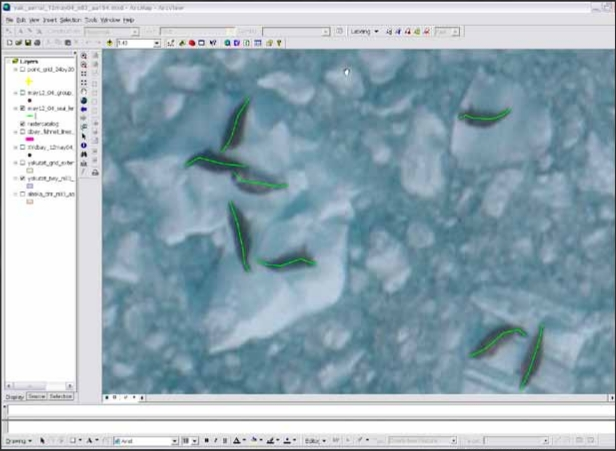
\includegraphics[width=5.0cm]{figure/aerialPhoto.jpeg} 
			\\
			\vspace{-1cm}
			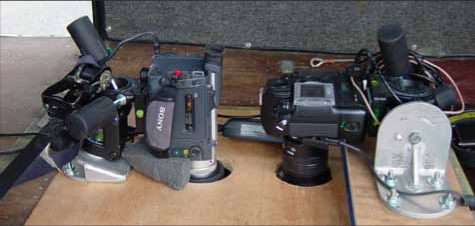
\includegraphics[width=4.6cm]{figure/cameras.jpeg} 


	\end{tabular}
\end{frame}

%-------------------------------------------------------------------------------
%                        Aerial Photos for Moose
%-------------------------------------------------------------------------------

\begin{frame}[fragile]
\frametitle{Aerial Photos for Moose}
	\begin{tabular} {p{5.0cm} p{5.0cm}}
	

			\vspace{-.2cm}
			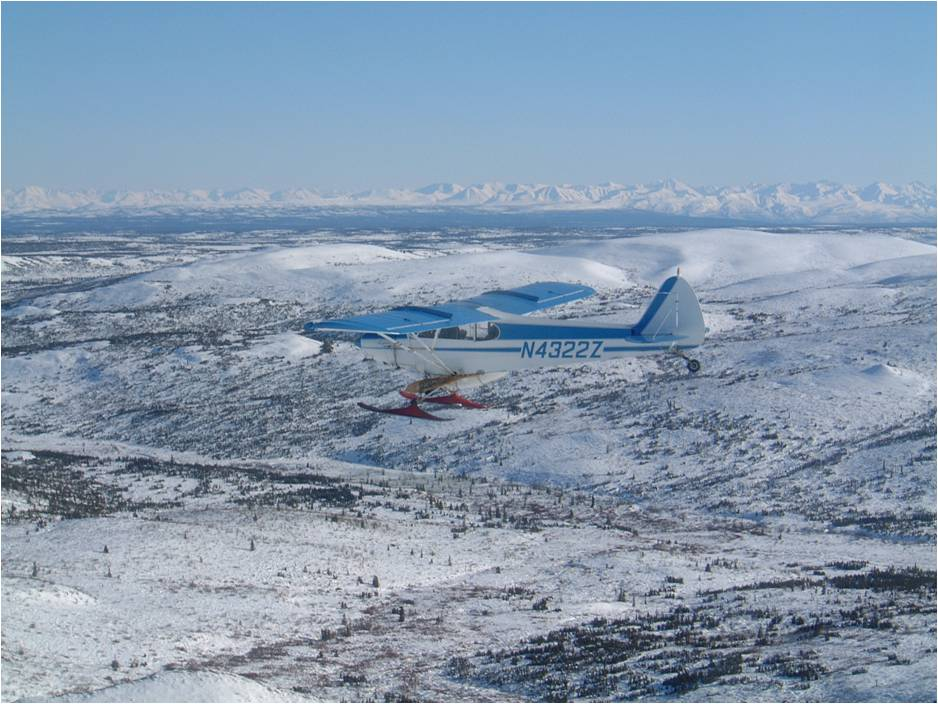
\includegraphics[width=4.4cm]{figure/SuperCub.jpeg}  &
			\vspace{1cm}
			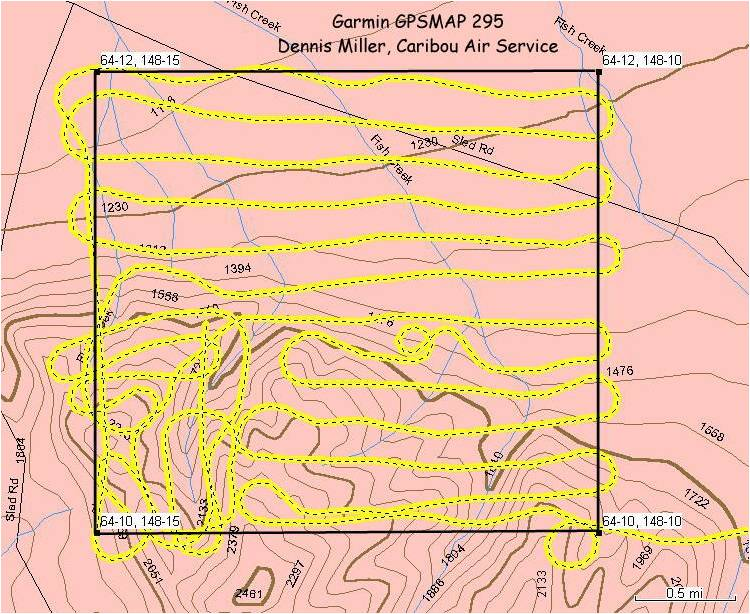
\includegraphics[width=5.0cm]{figure/vaporTrail.jpeg} 
			\\
			\vspace{-2.4cm}
			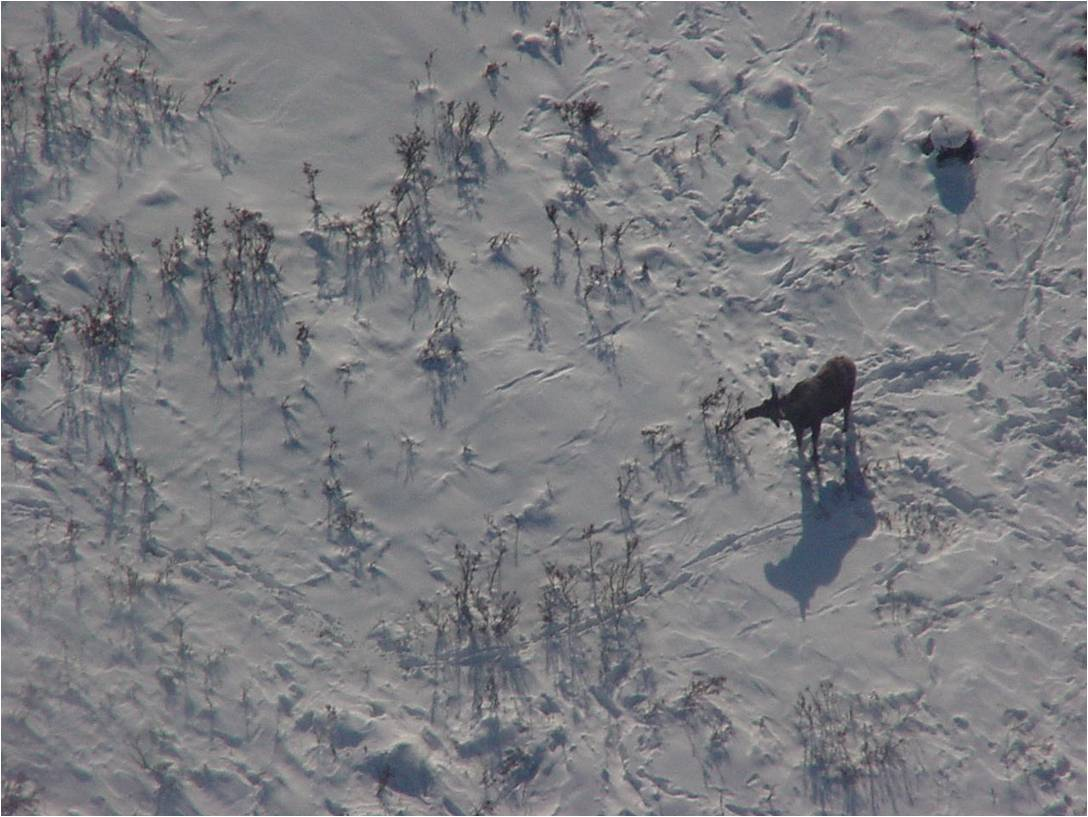
\includegraphics[width=4.4cm]{figure/Moose.jpeg} 


	\end{tabular}
\end{frame}

%-------------------------------------------------------------------------------
%                        INTRODUCTORY GRAPH
%-------------------------------------------------------------------------------
\begin{frame}[fragile]
\frametitle{Three Main Scenarios}

\begin{knitrout}\footnotesize
\definecolor{shadecolor}{rgb}{0.969, 0.969, 0.969}\color{fgcolor}
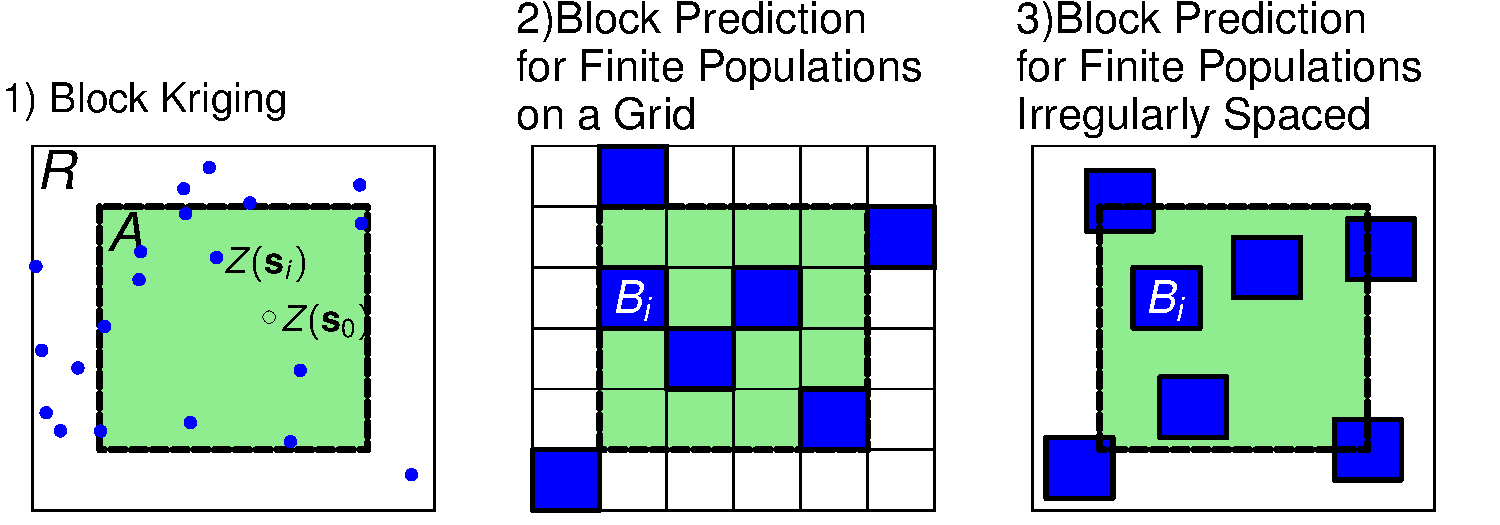
\includegraphics[width=\maxwidth]{figure/Introductory-plot} 

\end{knitrout}

\end{frame}
  
\end{document}
